\usecaseristoratore{Modifica lista ingredienti}
\label{usecase:Modifica lista ingredienti}

\begin{figure}[h]
	\centering
	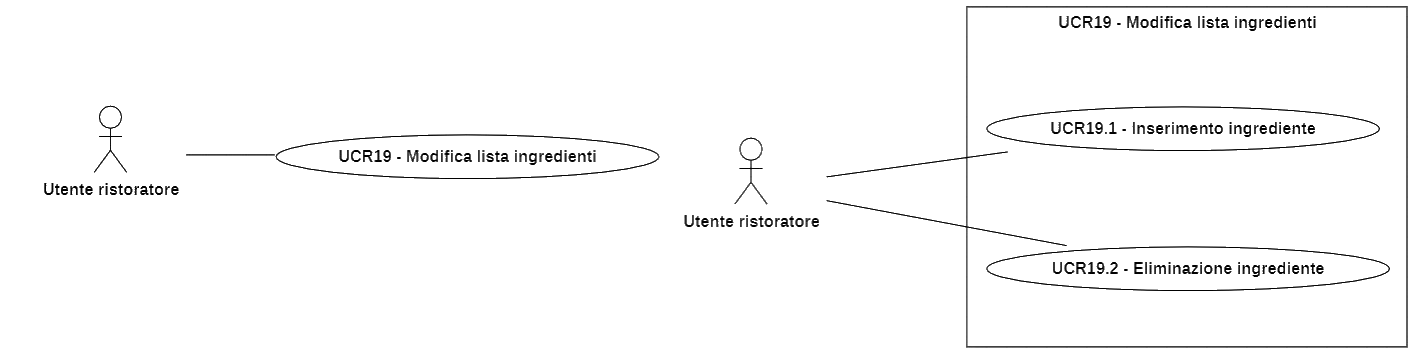
\includegraphics[width=0.9999\textwidth]{./uml/UCR19.png} 
	\caption{Modifica lista ingredienti}
	\label{fig:UCR19}
  \end{figure}

\begin{itemize}
	\item \textbf{Attore principale:} Utente ristoratore.

	\item \textbf{Precondizione:} L'Utente ristoratore ha effettuato l'accesso al Sistema (vedi \autoref{usecase:Effettua accesso}).

	\item \textbf{Postcondizione:} L'Utente ristoratore gestisce la lista degli ingredienti del proprio ristorante.


	\item \textbf{Scenario principale:}
	      \begin{enumerate}

		      \item L'Utente ristoratore può compiere le seguenti azioni per quanto riguarda la gestione della lista degli ingredienti:
		      \begin{itemize}
                \item Inserimento di un nuovo ingrediente (vedi \autoref{usecase:Inserimento ingrediente}).
                \item Eliminazione di un ingrediente (vedi \autoref{usecase:Eliminazione ingrediente}).
              \end{itemize}
		      \item Il Sistema registra le modifiche apporate alla lista ingredienti da parte del ristoratore.

	      \end{enumerate}
\end{itemize}

\subusecaseristoratore{Inserimento ingrediente}
\label{usecase:Inserimento ingrediente}
\begin{itemize}

	\item \textbf{Attore principale:} Utente ristoratore.

	\item \textbf{Precondizione:} L'Utente ristoratore si trova nella sezione di gestione della lista ingredienti (vedi \autoref{usecase:Modifica lista ingredienti}).

	\item \textbf{Postcondizione:} L'Utente ristoratore ha inserito un ingrediente nella lista.

	\item \textbf{Scenario principale:}
	\begin{enumerate}
		\item L'Utente ristoratore inserisce un nuovo ingrediente nella lista;
		\item Il Sistema aggiorna la lista con il nuovo ingrediente inserito dal ristoratore.
	\end{enumerate}

\end{itemize}

\subusecaseristoratore{Eliminazione ingrediente}
\label{usecase:Eliminazione ingrediente}
\begin{itemize}

	\item \textbf{Attore principale:} Utente ristoratore.

	\item \textbf{Precondizione:} L'Utente ristoratore si trova nella sezione di gestione della lista ingredienti (vedi \autoref{usecase:Modifica lista ingredienti}).

	\item \textbf{Postcondizione:} L'Utente ristoratore ha eliminato un ingrediente dalla lista.

	\item \textbf{Scenario principale:}
	\begin{enumerate}
		\item L'Utente ristoratore elimina un ingrediente dalla lista;
		\item Il Sistema aggiorna la lista con l'ingrediente che è stato eliminato dal ristoratore.
	\end{enumerate}

\end{itemize}
